
\subsection{Model description}
The model is constructed as a rate network of two populations of neurons \textit{U} and \textit{V}, the former representing the memory trace of the \textit{K} available options (\textit{i.e.} the bandits), and the latter the value of the options under the current policy.
More formally, the model is defined by a set of coupled ordinary differential equations (ODEs).
The first equation tracks the evolution of the neural activity $\textbf{u}$ of population \textit{U}, while the second tracks the activity $\textbf{v}$ of the population \textit{V}. The time constant $\tau$ is the same for both equations and it is set to $10$ms.

\begin{equation}
\begin{aligned}
    \tau \dot{\textbf{u}}&= -\textbf{u} + \textbf{W}^{VU}\phi_{v}(\textbf{v}) + \textbf{I}_{\text{ext}} \\
    \tau \dot{\textbf{v}}&= -\textbf{v} + \tilde{\textbf{W}}^{UV}\phi_{u}\textbf{u}
\end{aligned}
\end{equation}\label{eq:main}

\noindent The external input $\textbf{I}_{\text{ext}}$ is a constant input that is used to set the initial conditions of the neural activity $\textbf{u}$.
The activation functions $\phi_{v},\phi_{u}$ are applied to population $v$, and represent two distinct neural response function tailored to each population. They have been chosen to be a step-function with threshold $\theta_{v},\theta_{v}$ applied to a generalized sigmoid with gain $g_{v},g_{u}$ and offset $s_{v},s_{u}$.

\begin{figure}[ht]
    \centering
    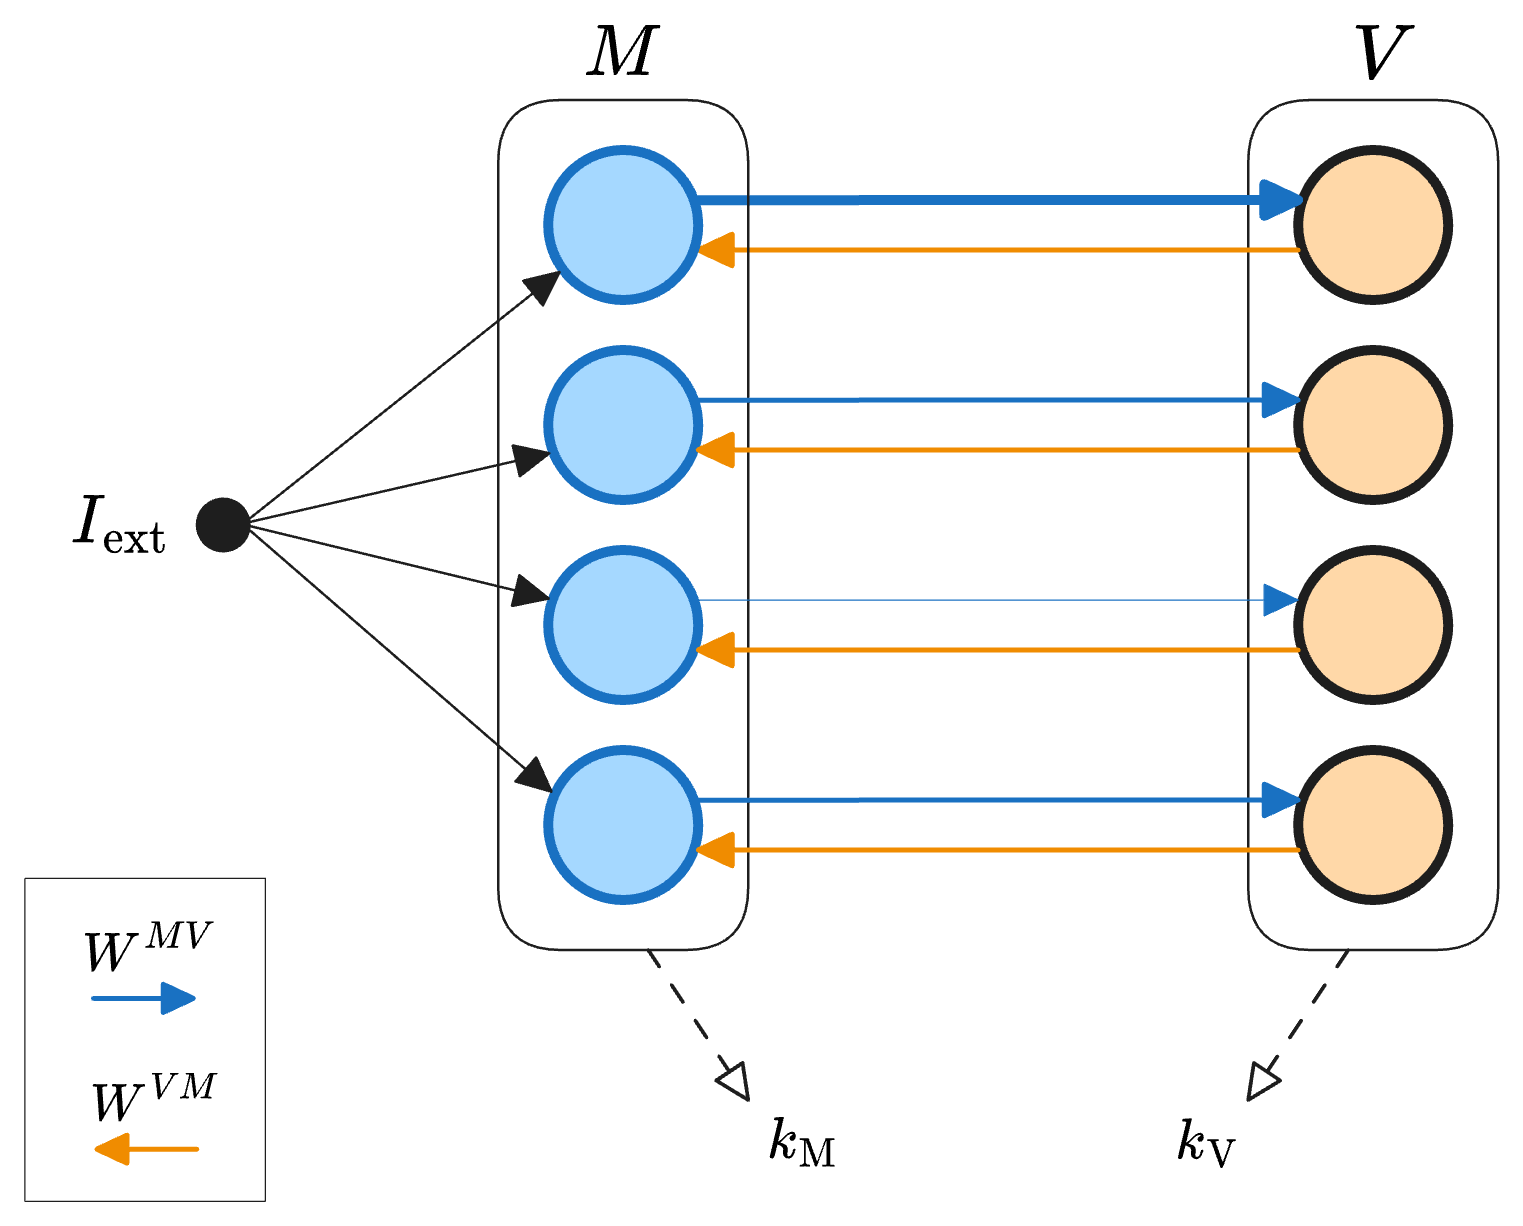
\includegraphics[width=0.6\textwidth]{figures/minb_architecture.png}
    \caption{\textsc{Model architecture} - \textit{The model is composed of a layer $U$ (blue), receiving a feedfoward input $I_{\text{ext}}$, a layer $V$ (orange), and connections $\textbf{W}^{UV}$ and $\textbf{W}^{VU}$. Additionally, two indexes $k_{U}, k_{V}$  can be extracted from the layers and
    corresponds to the selection made by the two populations as $k_{U}=\text{argmax}_{k} \{\textbf{u}\}$, $k_{V}=\text{argmax}_{k} \{\textbf{v}\}$.}}
    \label{fig:main_architecture}
\end{figure}

\noindent Importantly, the two layers are not fully connected and the matrices are diagonal.
More in detail, the weight matrix $\textbf{W}^{VU}$ is simply made of $1$s, while $\tilde{\textbf{W}}^{UV}$ is a function of the actual weights $\Phi_{v}(\textbf{W}^{UV})$ and it represents the contribution of the active options $\textbf{u}$ to the value representation $\textbf{v}$, it is thus referred to as \textit{option value function}.
The function $\Phi_{v}$ is defined a weighted sum of a generalized sigmoid and a Gaussian, whose shape is characterized by a bell curve smoothly settling to a constant value. For details see in the appendinx \ref{sec:appendix}.
Since the exact values of the model hyperparameters are optimized through an evolution, our motivation behind the structure of $\Phi_{v}$ is to be agnostic about its final form, and allow competition or integration of two distinct traits of the function shape.
One is a smooth transition to a plateau value with a certain steepness (or gain), which can represent a saturation once a threshold is crossed, such feature has been reporeted for both biological and artificial neurons \cite{ockerFlexibleNeuralConnectivity2020, apicellaSurveyModernTrainable2021}.
The other is a bell-shaped curve with a defined center and width, which can allow for placing emphasis on values only within a given window and modulate information transfer \cite{millerCombinedMechanismsNeural2019}.

\subsubsection{Option selection}
The decision-making process within a single round is structured in two distinct phases. Initially, the model receives a constant external input targeting all neurons in the memory population \textit{U} equally.
During this phase, $\textbf{I}_{\text{ext}}$ works as an equilibrium value while the reciprocal interactions with population \textit{V} push $\textbf{u}$ to different values, depending on the current policy encoded in $\tilde{\textbf{W}}^{UV}$.
Importantly, the weights $\textbf{W}^{UV}$ are initialized to zero, and thus the input from $U$ to $V$ is uniform. This approach ensures the absence of biases towards any arm by having all weights equal, and corresponds to a completely untrained network.
After a fixed amount of time $\sim 2 \text{s}$, the second phase begins. Here, the external input is removed and the model is left to evolve autonomously, and since there are no recurrent connections in neither population the dynamics are entirely driven by their coupling.
A selection $k$ is sampled after another fixed amount of time $\sim 5 \text{s}$, and it is defined according to the following rule:

\begin{equation*}
    k =
    \left\{
        \begin{array}{ll}
            \text{argmax}_{k}\{\textbf{v}\} & \text{\textit{if}}\; \text{argmax}_{k} \{\textbf{v}\} = \text{argmax}_{k} \{\textbf{u}\} \\
            \text{random}(K) & \text{\textit{otherwise}}
        \end{array}
    \right.
\end{equation*}

\noindent The selection rule is simple: if the value representation $\textbf{v}$ is in agreement with the memory trace $\textbf{u}$, then the option with the highest value is selected. Otherwise, a random option is chosen.
This rule is a way to express the exploration-exploitation trade-off, and it is dependent on the current policy $\tilde{\textbf{W}}^{UV}$. \\ Below \ref{alg:decision1}, is reported the pseudo-code for algorithm behind the selection process, which is applied during each round $t$.

% --- ALGORITHM
\begin{algorithm}[ht]
\caption{Two-phases option selection process}
\label{alg:decision}
\SetAlgoLined
\KwIn{External input $\textbf{I}_{\text{ext}}$, population $\textbf{u}$, population $\textbf{v}$, weights $\tilde{\textbf{W}}^{UV}$}
\KwOut{Selected action $k$}

\SetKwComment{Comment}{// }{ }

\textbf{Phase 1:} \textit{external input} \Comment*[r]{Duration: $\sim$2s}
Define constant $\textbf{I}_{\text{ext}}$\;
Update populations $\textbf{u}, \textbf{v}$ according to \ref{eq:main}\;

\textbf{Phase 2:} \textit{autonomous evolution} \Comment*[r]{Duration: $\sim$2s}
Remove external input $\textbf{I}_{\text{ext}}$\;
Let system evolve through population coupling according to \ref{eq:main}\;

\textbf{Selection process:}\;
$k_{u} \gets \text{argmax}_{k}\{\textbf{u}\}$\;
$k_{v} \gets \text{argmax}_{k}\{\textbf{v}\}$\;
\eIf{$k_{u} = k_{v}$}{
    $k \gets k_{v}$ \Comment*[r]{Exploitation}}{
    $k \gets \text{random}(K)$ \Comment*[r]{Exploration}
}
\Return $k$
\end{algorithm}\label{alg:decision1}

\noindent According to the values of the policy's parameters, the behaviour of the model displays periods of exploration followed by a steady exploitation, which can be reverted in case of a change in the environment's reward distribution.

% selections over time
% \begin{figure}[ht]
%     \centering
%     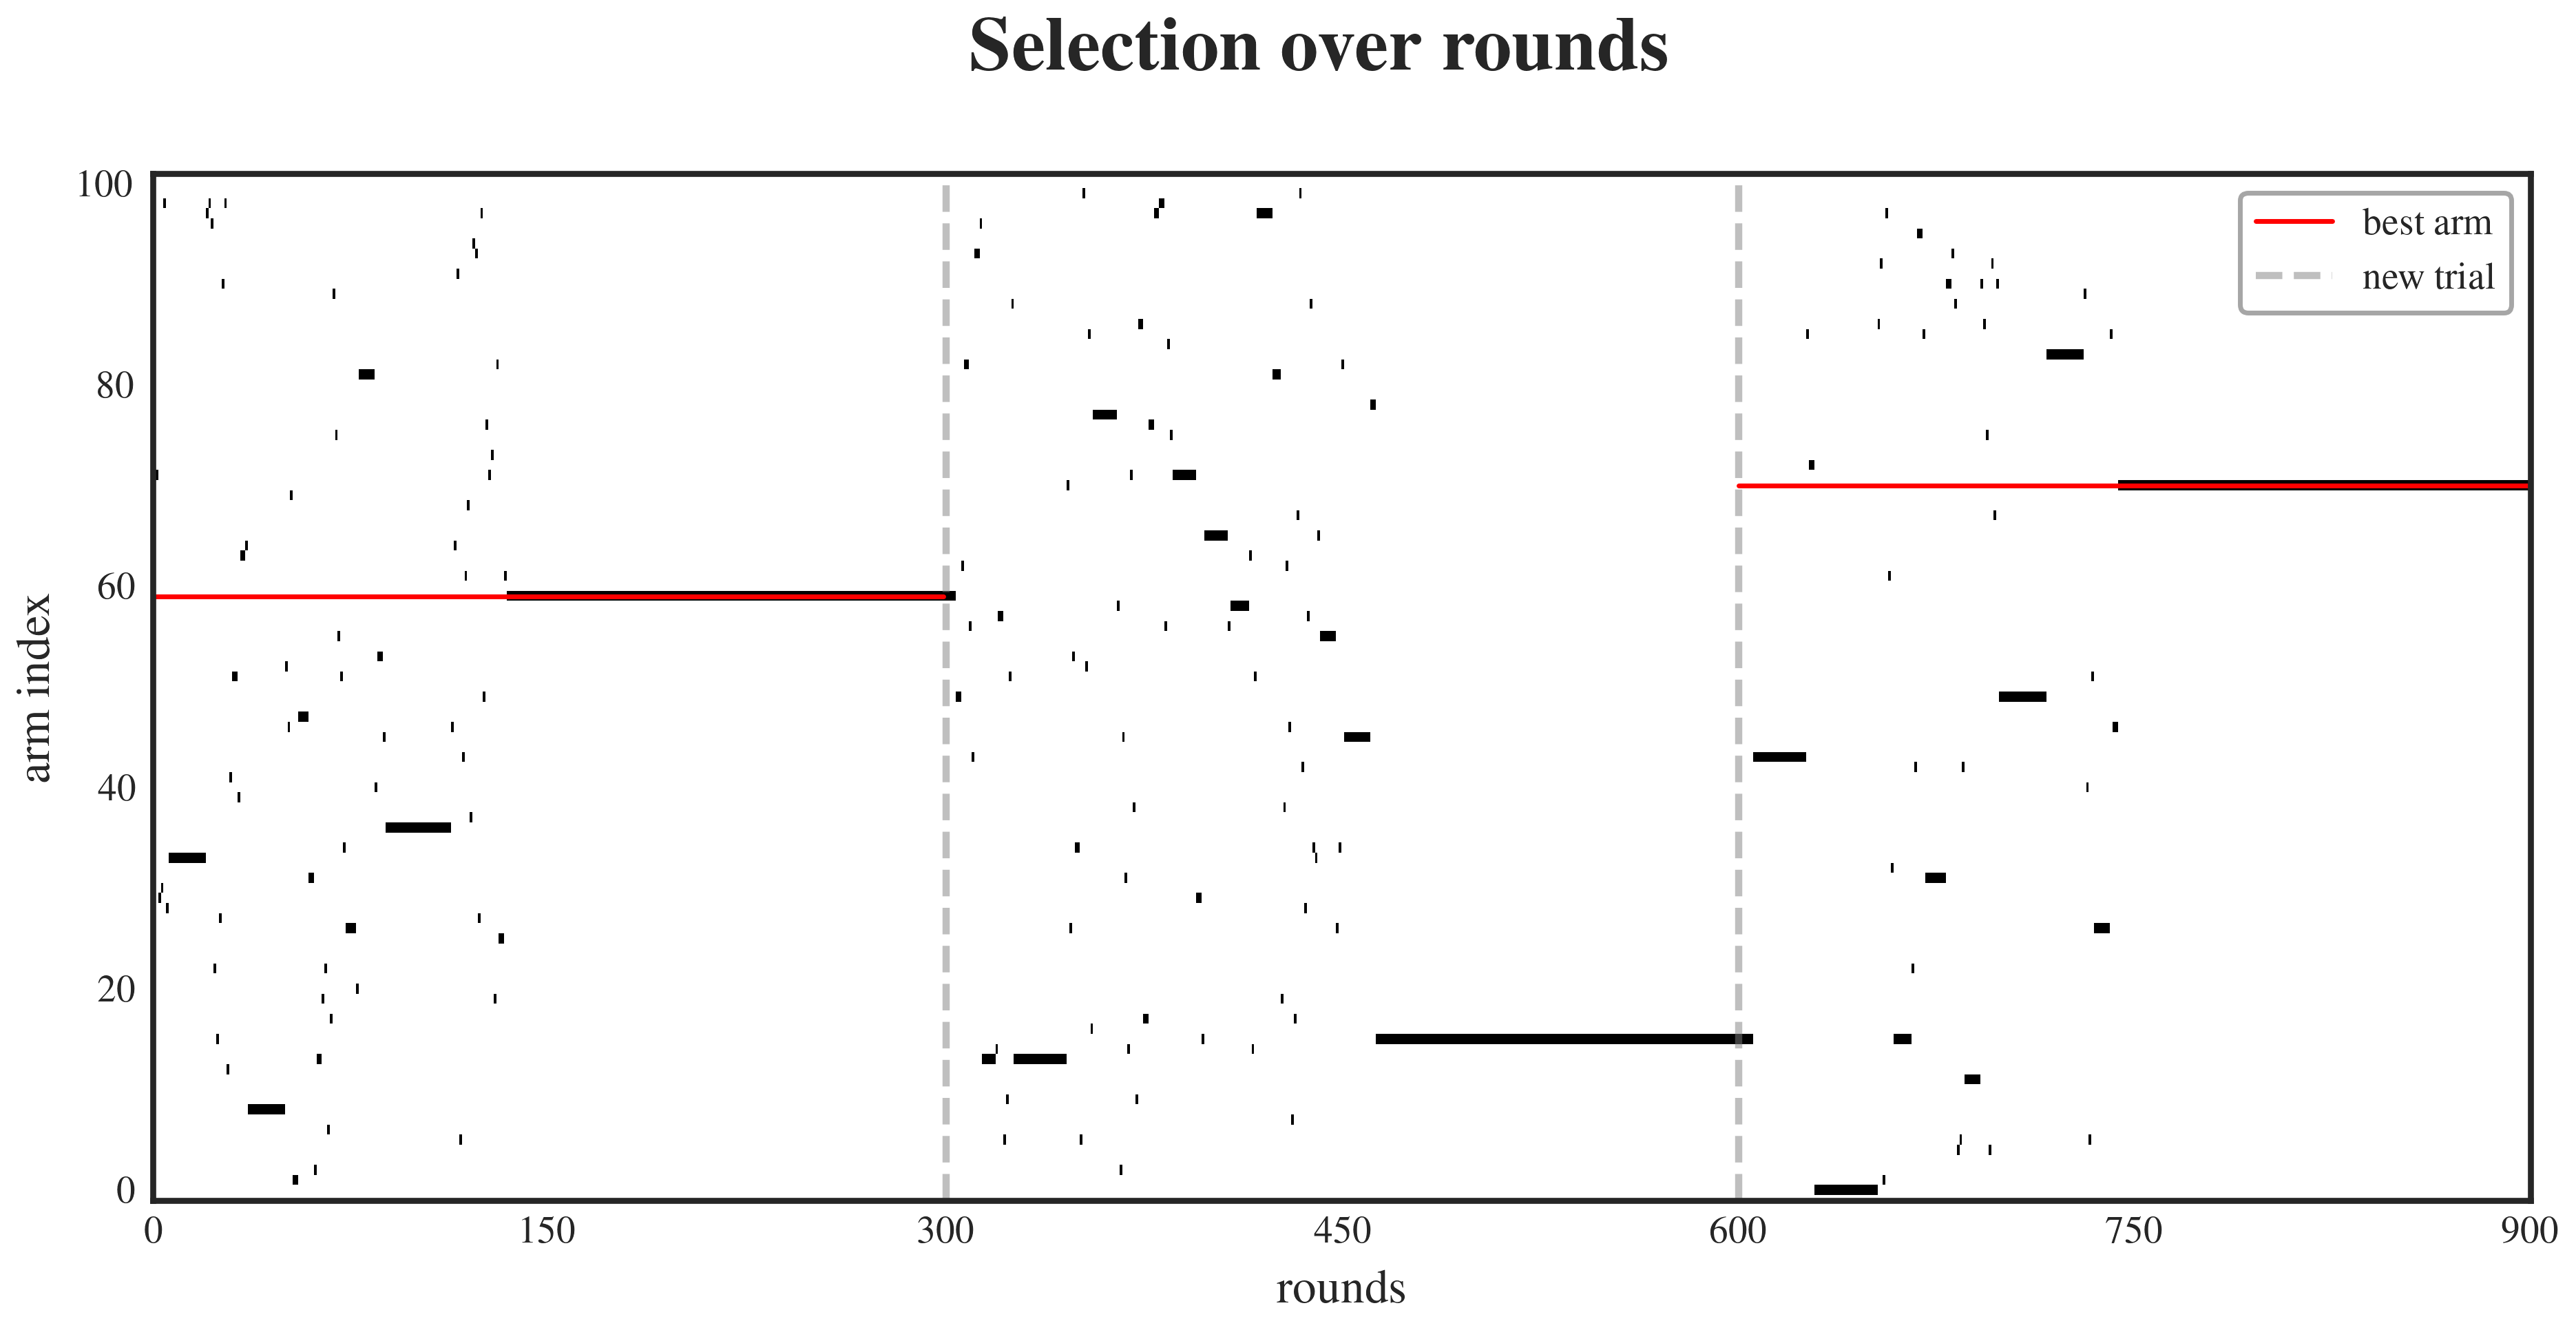
\includegraphics[width=0.9\textwidth]{figures/selections_2.png}
%     \caption{\textsc{Selection evolution over rounds} - \textit{the y-axis represents the available arms, while the x-axis the number of rounds, with the dotted vertical lines indicating the start of a new trial with 300 rounds each.
% The model selections are the black vertical lines for an arm and a round. The red horizontal lines signal the arm with the highest reward probability, representing the best option.}}
%     \label{fig:sel1}
% \end{figure}


\subsection{Learning}
Given a selected option $k$, the environment (set of bandits) samples and returns a reward $R\in \{0, 1\}$ with probability $p_{k}$.
Then, the connections $\textbf{W}^{UV}$ for the neuron corresponding to the option $k$ are updated according to the following plasticity rule:

\begin{equation}
    \Delta \textbf{W}^{UV}_{k} = \tilde{\eta}_{k} \left(R\cdot w^{+}- \textbf{W}^{UV}_{k}\right)
\end{equation}

\noindent where $w^{+}$ is a constant maximum synaptic weight, while $\tilde{\eta}_{k}$ is the learning rate for the option $k$ determined by a function $\Phi_{\eta}$ of the current weights $\textbf{W}^{UV}_{k}$, referred to as \textit{learning rate function}.

The shape of $\Phi_{\eta}$ is again a Gaussian-sigmoid but with different parameters, giving evolution the opportunity to combine the shape traits of plateau and bell-shaped tuning in a task-efficient manner.
In particular, these features can be combined so to define mechanisms of synapse-type specific plasticity as a function of the current synaptic strenght \cite{larsenSynapsetypespecificPlasticityLocal2015}, as well the application of other useful homeostatic constraints with computational advantages, such as synaptic scaling and proportional updates \cite{citriSynapticPlasticityMultiple2008, kennedySynapticSignalingLearning2016, samavatSynapticInformationStorage2024}.


